% Options for packages loaded elsewhere
\PassOptionsToPackage{unicode}{hyperref}
\PassOptionsToPackage{hyphens}{url}
\documentclass[
]{article}
\usepackage{xcolor}
\usepackage[margin=1in]{geometry}
\usepackage{amsmath,amssymb}
\setcounter{secnumdepth}{-\maxdimen} % remove section numbering
\usepackage{iftex}
\ifPDFTeX
  \usepackage[T1]{fontenc}
  \usepackage[utf8]{inputenc}
  \usepackage{textcomp} % provide euro and other symbols
\else % if luatex or xetex
  \usepackage{unicode-math} % this also loads fontspec
  \defaultfontfeatures{Scale=MatchLowercase}
  \defaultfontfeatures[\rmfamily]{Ligatures=TeX,Scale=1}
\fi
\usepackage{lmodern}
\ifPDFTeX\else
  % xetex/luatex font selection
\fi
% Use upquote if available, for straight quotes in verbatim environments
\IfFileExists{upquote.sty}{\usepackage{upquote}}{}
\IfFileExists{microtype.sty}{% use microtype if available
  \usepackage[]{microtype}
  \UseMicrotypeSet[protrusion]{basicmath} % disable protrusion for tt fonts
}{}
\makeatletter
\@ifundefined{KOMAClassName}{% if non-KOMA class
  \IfFileExists{parskip.sty}{%
    \usepackage{parskip}
  }{% else
    \setlength{\parindent}{0pt}
    \setlength{\parskip}{6pt plus 2pt minus 1pt}}
}{% if KOMA class
  \KOMAoptions{parskip=half}}
\makeatother
\usepackage{color}
\usepackage{fancyvrb}
\newcommand{\VerbBar}{|}
\newcommand{\VERB}{\Verb[commandchars=\\\{\}]}
\DefineVerbatimEnvironment{Highlighting}{Verbatim}{commandchars=\\\{\}}
% Add ',fontsize=\small' for more characters per line
\usepackage{framed}
\definecolor{shadecolor}{RGB}{248,248,248}
\newenvironment{Shaded}{\begin{snugshade}}{\end{snugshade}}
\newcommand{\AlertTok}[1]{\textcolor[rgb]{0.94,0.16,0.16}{#1}}
\newcommand{\AnnotationTok}[1]{\textcolor[rgb]{0.56,0.35,0.01}{\textbf{\textit{#1}}}}
\newcommand{\AttributeTok}[1]{\textcolor[rgb]{0.13,0.29,0.53}{#1}}
\newcommand{\BaseNTok}[1]{\textcolor[rgb]{0.00,0.00,0.81}{#1}}
\newcommand{\BuiltInTok}[1]{#1}
\newcommand{\CharTok}[1]{\textcolor[rgb]{0.31,0.60,0.02}{#1}}
\newcommand{\CommentTok}[1]{\textcolor[rgb]{0.56,0.35,0.01}{\textit{#1}}}
\newcommand{\CommentVarTok}[1]{\textcolor[rgb]{0.56,0.35,0.01}{\textbf{\textit{#1}}}}
\newcommand{\ConstantTok}[1]{\textcolor[rgb]{0.56,0.35,0.01}{#1}}
\newcommand{\ControlFlowTok}[1]{\textcolor[rgb]{0.13,0.29,0.53}{\textbf{#1}}}
\newcommand{\DataTypeTok}[1]{\textcolor[rgb]{0.13,0.29,0.53}{#1}}
\newcommand{\DecValTok}[1]{\textcolor[rgb]{0.00,0.00,0.81}{#1}}
\newcommand{\DocumentationTok}[1]{\textcolor[rgb]{0.56,0.35,0.01}{\textbf{\textit{#1}}}}
\newcommand{\ErrorTok}[1]{\textcolor[rgb]{0.64,0.00,0.00}{\textbf{#1}}}
\newcommand{\ExtensionTok}[1]{#1}
\newcommand{\FloatTok}[1]{\textcolor[rgb]{0.00,0.00,0.81}{#1}}
\newcommand{\FunctionTok}[1]{\textcolor[rgb]{0.13,0.29,0.53}{\textbf{#1}}}
\newcommand{\ImportTok}[1]{#1}
\newcommand{\InformationTok}[1]{\textcolor[rgb]{0.56,0.35,0.01}{\textbf{\textit{#1}}}}
\newcommand{\KeywordTok}[1]{\textcolor[rgb]{0.13,0.29,0.53}{\textbf{#1}}}
\newcommand{\NormalTok}[1]{#1}
\newcommand{\OperatorTok}[1]{\textcolor[rgb]{0.81,0.36,0.00}{\textbf{#1}}}
\newcommand{\OtherTok}[1]{\textcolor[rgb]{0.56,0.35,0.01}{#1}}
\newcommand{\PreprocessorTok}[1]{\textcolor[rgb]{0.56,0.35,0.01}{\textit{#1}}}
\newcommand{\RegionMarkerTok}[1]{#1}
\newcommand{\SpecialCharTok}[1]{\textcolor[rgb]{0.81,0.36,0.00}{\textbf{#1}}}
\newcommand{\SpecialStringTok}[1]{\textcolor[rgb]{0.31,0.60,0.02}{#1}}
\newcommand{\StringTok}[1]{\textcolor[rgb]{0.31,0.60,0.02}{#1}}
\newcommand{\VariableTok}[1]{\textcolor[rgb]{0.00,0.00,0.00}{#1}}
\newcommand{\VerbatimStringTok}[1]{\textcolor[rgb]{0.31,0.60,0.02}{#1}}
\newcommand{\WarningTok}[1]{\textcolor[rgb]{0.56,0.35,0.01}{\textbf{\textit{#1}}}}
\usepackage{graphicx}
\makeatletter
\newsavebox\pandoc@box
\newcommand*\pandocbounded[1]{% scales image to fit in text height/width
  \sbox\pandoc@box{#1}%
  \Gscale@div\@tempa{\textheight}{\dimexpr\ht\pandoc@box+\dp\pandoc@box\relax}%
  \Gscale@div\@tempb{\linewidth}{\wd\pandoc@box}%
  \ifdim\@tempb\p@<\@tempa\p@\let\@tempa\@tempb\fi% select the smaller of both
  \ifdim\@tempa\p@<\p@\scalebox{\@tempa}{\usebox\pandoc@box}%
  \else\usebox{\pandoc@box}%
  \fi%
}
% Set default figure placement to htbp
\def\fps@figure{htbp}
\makeatother
\setlength{\emergencystretch}{3em} % prevent overfull lines
\providecommand{\tightlist}{%
  \setlength{\itemsep}{0pt}\setlength{\parskip}{0pt}}
\usepackage{bookmark}
\IfFileExists{xurl.sty}{\usepackage{xurl}}{} % add URL line breaks if available
\urlstyle{same}
\hypersetup{
  pdftitle={Combined\_Growth\_and\_Fecundity\_Plots},
  pdfauthor={Stephen R. Proulx},
  hidelinks,
  pdfcreator={LaTeX via pandoc}}

\title{Combined\_Growth\_and\_Fecundity\_Plots}
\author{Stephen R. Proulx}
\date{2026-03-20}

\begin{document}
\maketitle

re-usable features for growth data

plot functions

\subsection{Fitness data}\label{fitness-data}

\pandocbounded{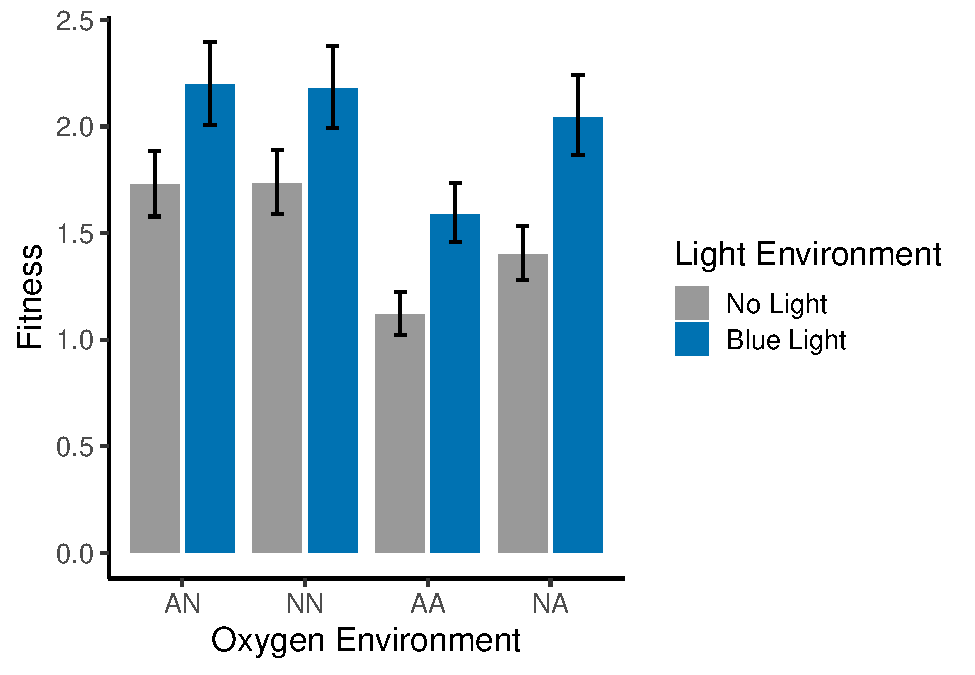
\includegraphics[keepaspectratio]{03_Combined_Growth_Fecundity_Plots_files/figure-latex/growth_plot_anc_growth_by_matcue_intervals_from_state_only-1.pdf}}

\pandocbounded{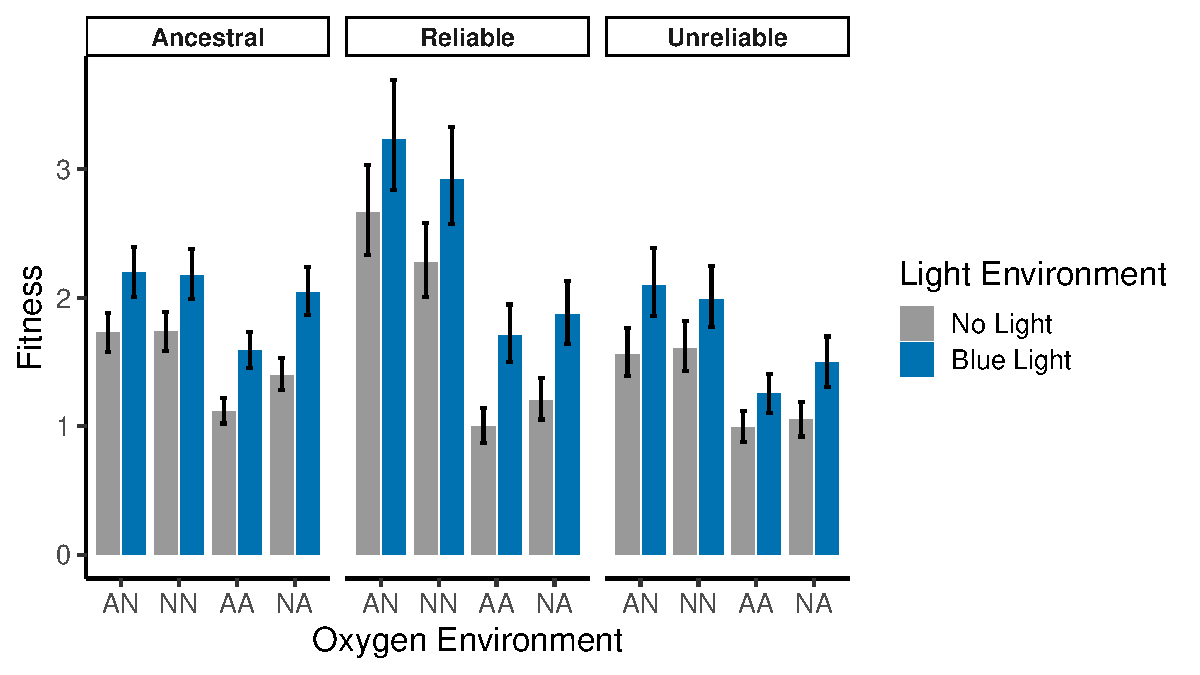
\includegraphics[keepaspectratio]{03_Combined_Growth_Fecundity_Plots_files/figure-latex/growth_plot_anc_rel_unrel_growth_by_matcue_intervals_state_only-1.pdf}}

This figure shows the difference in R0 from the ancestral for reliable
and unreliable. i.e.~R0\_rel-R0\_anc and R0\_unrel-R0\_anc. So the pop
growth parameters are calculated, exp'ed, and then difference taken.

\pandocbounded{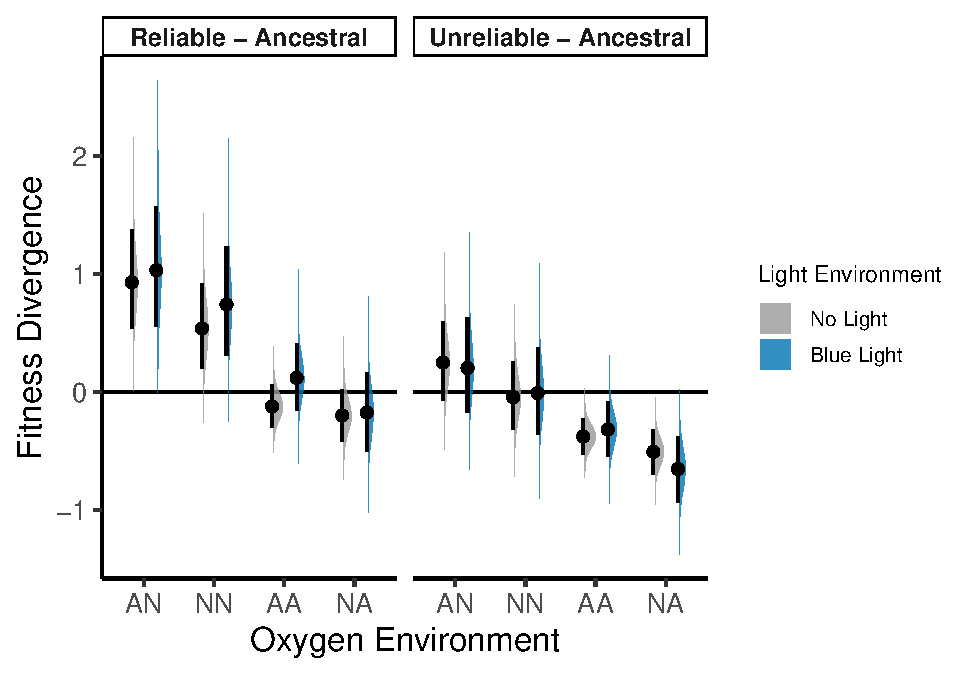
\includegraphics[keepaspectratio]{03_Combined_Growth_Fecundity_Plots_files/figure-latex/growth_plot_rel_unrel_minus_anc_growth_contrast_boxplot_style_fecundity_like-1.pdf}}

Plot the cue effect. This finds the R0 values for each state for each
treatment, then subtracts Rel-Anc or Unrel-Anc, so outcome is difference
in R0

\pandocbounded{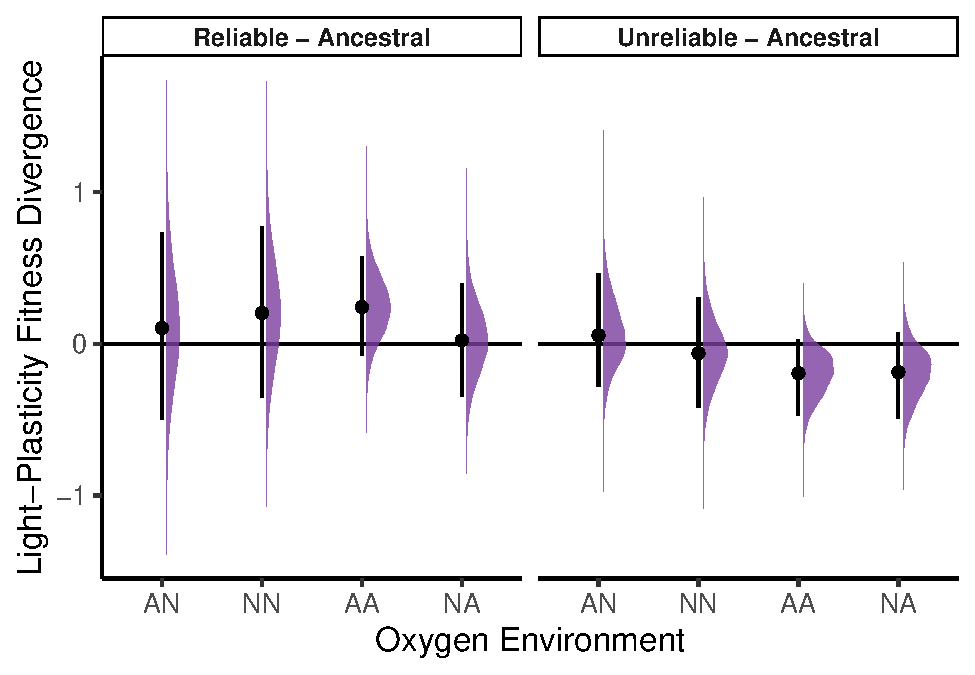
\includegraphics[keepaspectratio]{03_Combined_Growth_Fecundity_Plots_files/figure-latex/growth_plot_rel_unrel_vs_anc_cue_effect_contrast_boxplot_style_combined-1.pdf}}

this is the difference of the difference between Rel and Unrel. First
calculate the difference in R0 based on cue for Rel, and Unrel. Then do
Rel-Unrel of that difference.

\pandocbounded{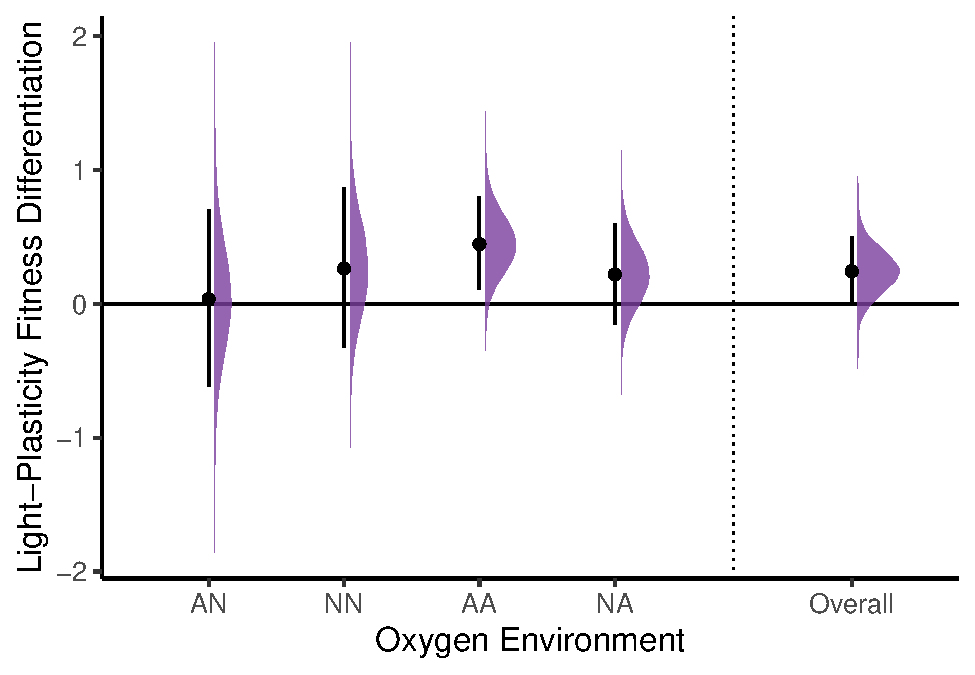
\includegraphics[keepaspectratio]{03_Combined_Growth_Fecundity_Plots_files/figure-latex/growth_plot_rel_vs_unrel_cue_effect_difference_contrast_boxplot_style-1.pdf}}

Here the contrasts in mean log fitness are calculated on log scale
(because it is geo mean of R0). We then plot fixed-reference changes on
the R0 scale so they can be seen in terms of number of offspring. We do
this by taking exp( Anc + 1/2 diff in log fit due to evo treat)-exp( Anc
- 1/2 diff in log fit due to evo treat)

\pandocbounded{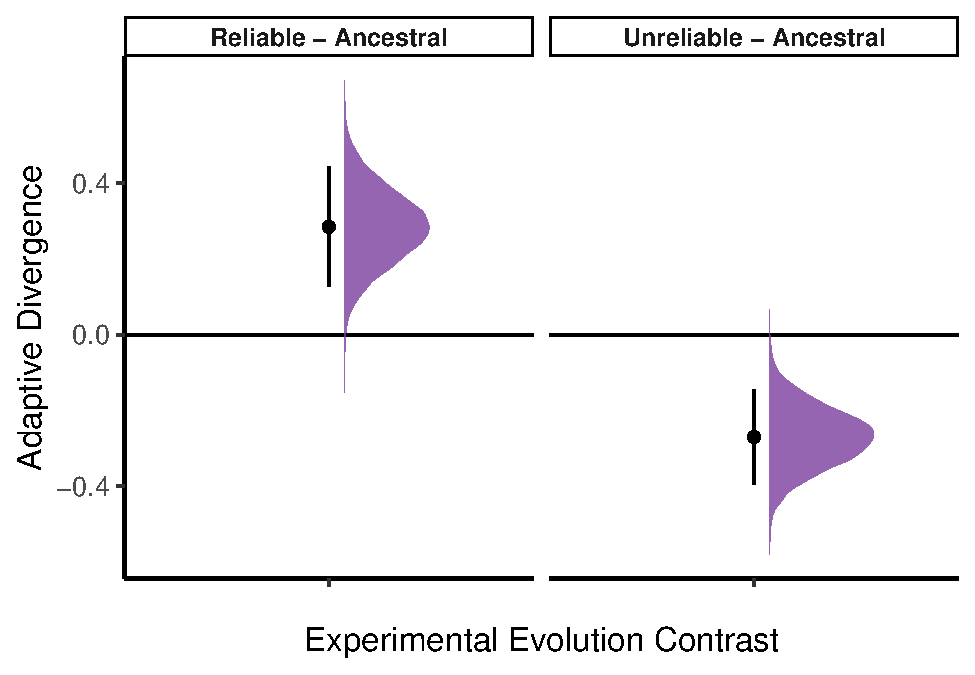
\includegraphics[keepaspectratio]{03_Combined_Growth_Fecundity_Plots_files/figure-latex/geo_mean -1.pdf}}

Showing the average log fitness transformed to the natural R0 scale.
i.e.~geo mean of R0

\pandocbounded{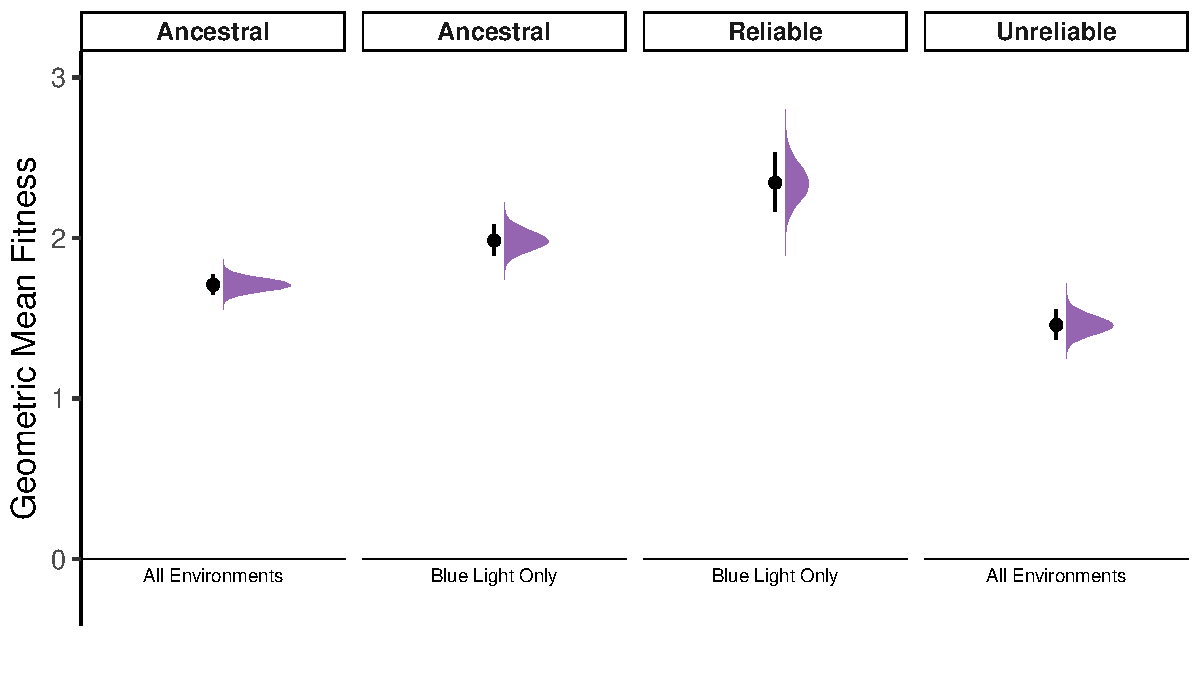
\includegraphics[keepaspectratio]{03_Combined_Growth_Fecundity_Plots_files/figure-latex/growth_plot_average_growth_custom_blue_rel_all_unrel-1.pdf}}

Here we go to the natural scale and then take the contrast between cue
and no cue R0 averaged across mat ox states

\pandocbounded{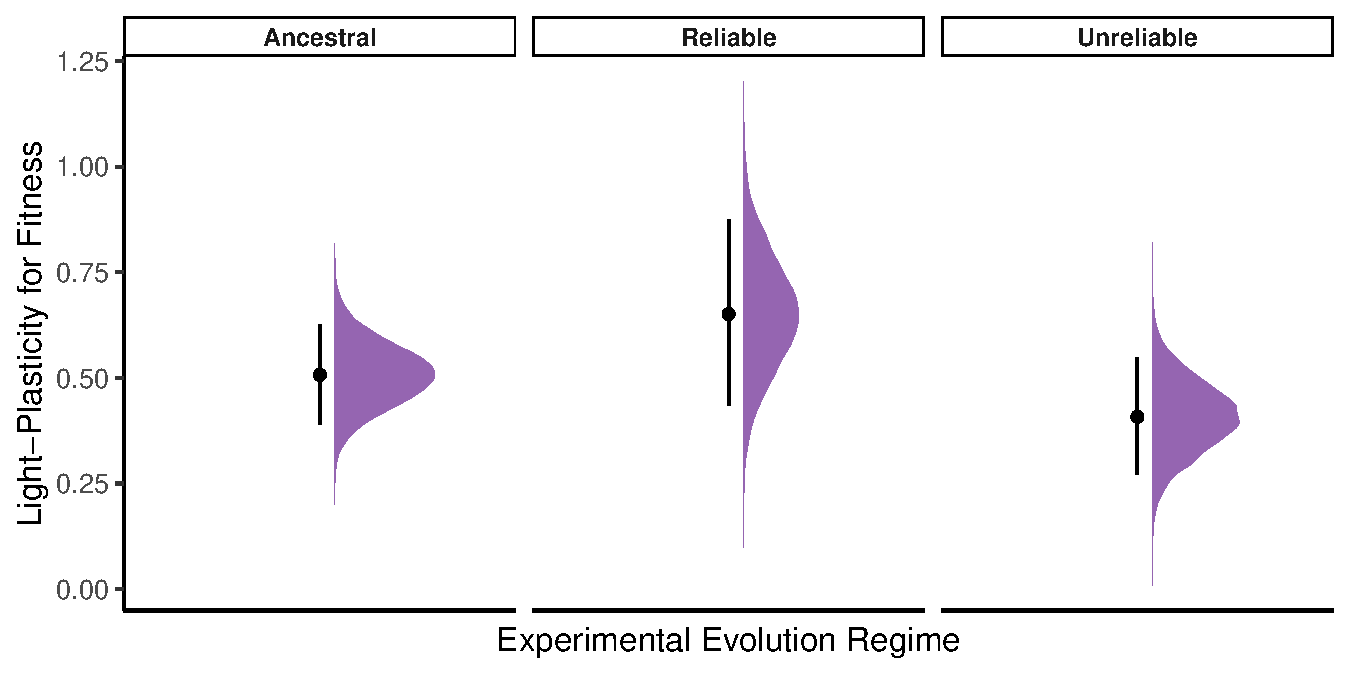
\includegraphics[keepaspectratio]{03_Combined_Growth_Fecundity_Plots_files/figure-latex/growth_plot_overall_cue_contrast_averaged_across_mat-1.pdf}}

Difference in cue effect on R0 between Rel and Unrel

\pandocbounded{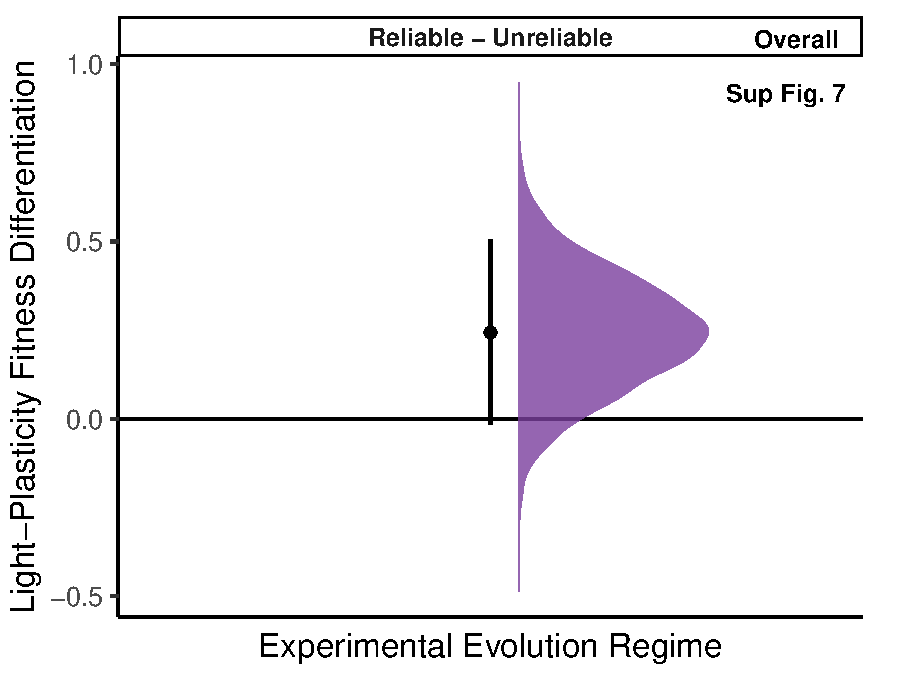
\includegraphics[keepaspectratio]{03_Combined_Growth_Fecundity_Plots_files/figure-latex/growth_plot_rel_vs_unrel_overall_cue_contrast-1.pdf}}

Figure out exactly how much of the posterior is above 0. 6.3\% is below
zero.

\begin{Shaded}
\begin{Highlighting}[]
\NormalTok{df\_draws }\SpecialCharTok{\%\textgreater{}\%}
  \FunctionTok{group\_by}\NormalTok{(contrast\_box, x\_dummy) }\SpecialCharTok{\%\textgreater{}\%}
  \FunctionTok{summarise}\NormalTok{(}
    \AttributeTok{med =} \FunctionTok{median}\NormalTok{(diff\_fit),}
    \AttributeTok{lo =} \FunctionTok{quantile}\NormalTok{(diff\_fit, }\FloatTok{0.063}\NormalTok{),}
    \AttributeTok{.groups =} \StringTok{"drop"}
\NormalTok{  )}
\end{Highlighting}
\end{Shaded}

\begin{verbatim}
## # A tibble: 1 x 4
##   contrast_box          x_dummy   med       lo
##   <fct>                 <fct>   <dbl>    <dbl>
## 1 Reliable - Unreliable ""      0.244 -0.00482
\end{verbatim}

Analyze the total difference in fitness under the blue light cue between
Reliable and Unreliable:
\pandocbounded{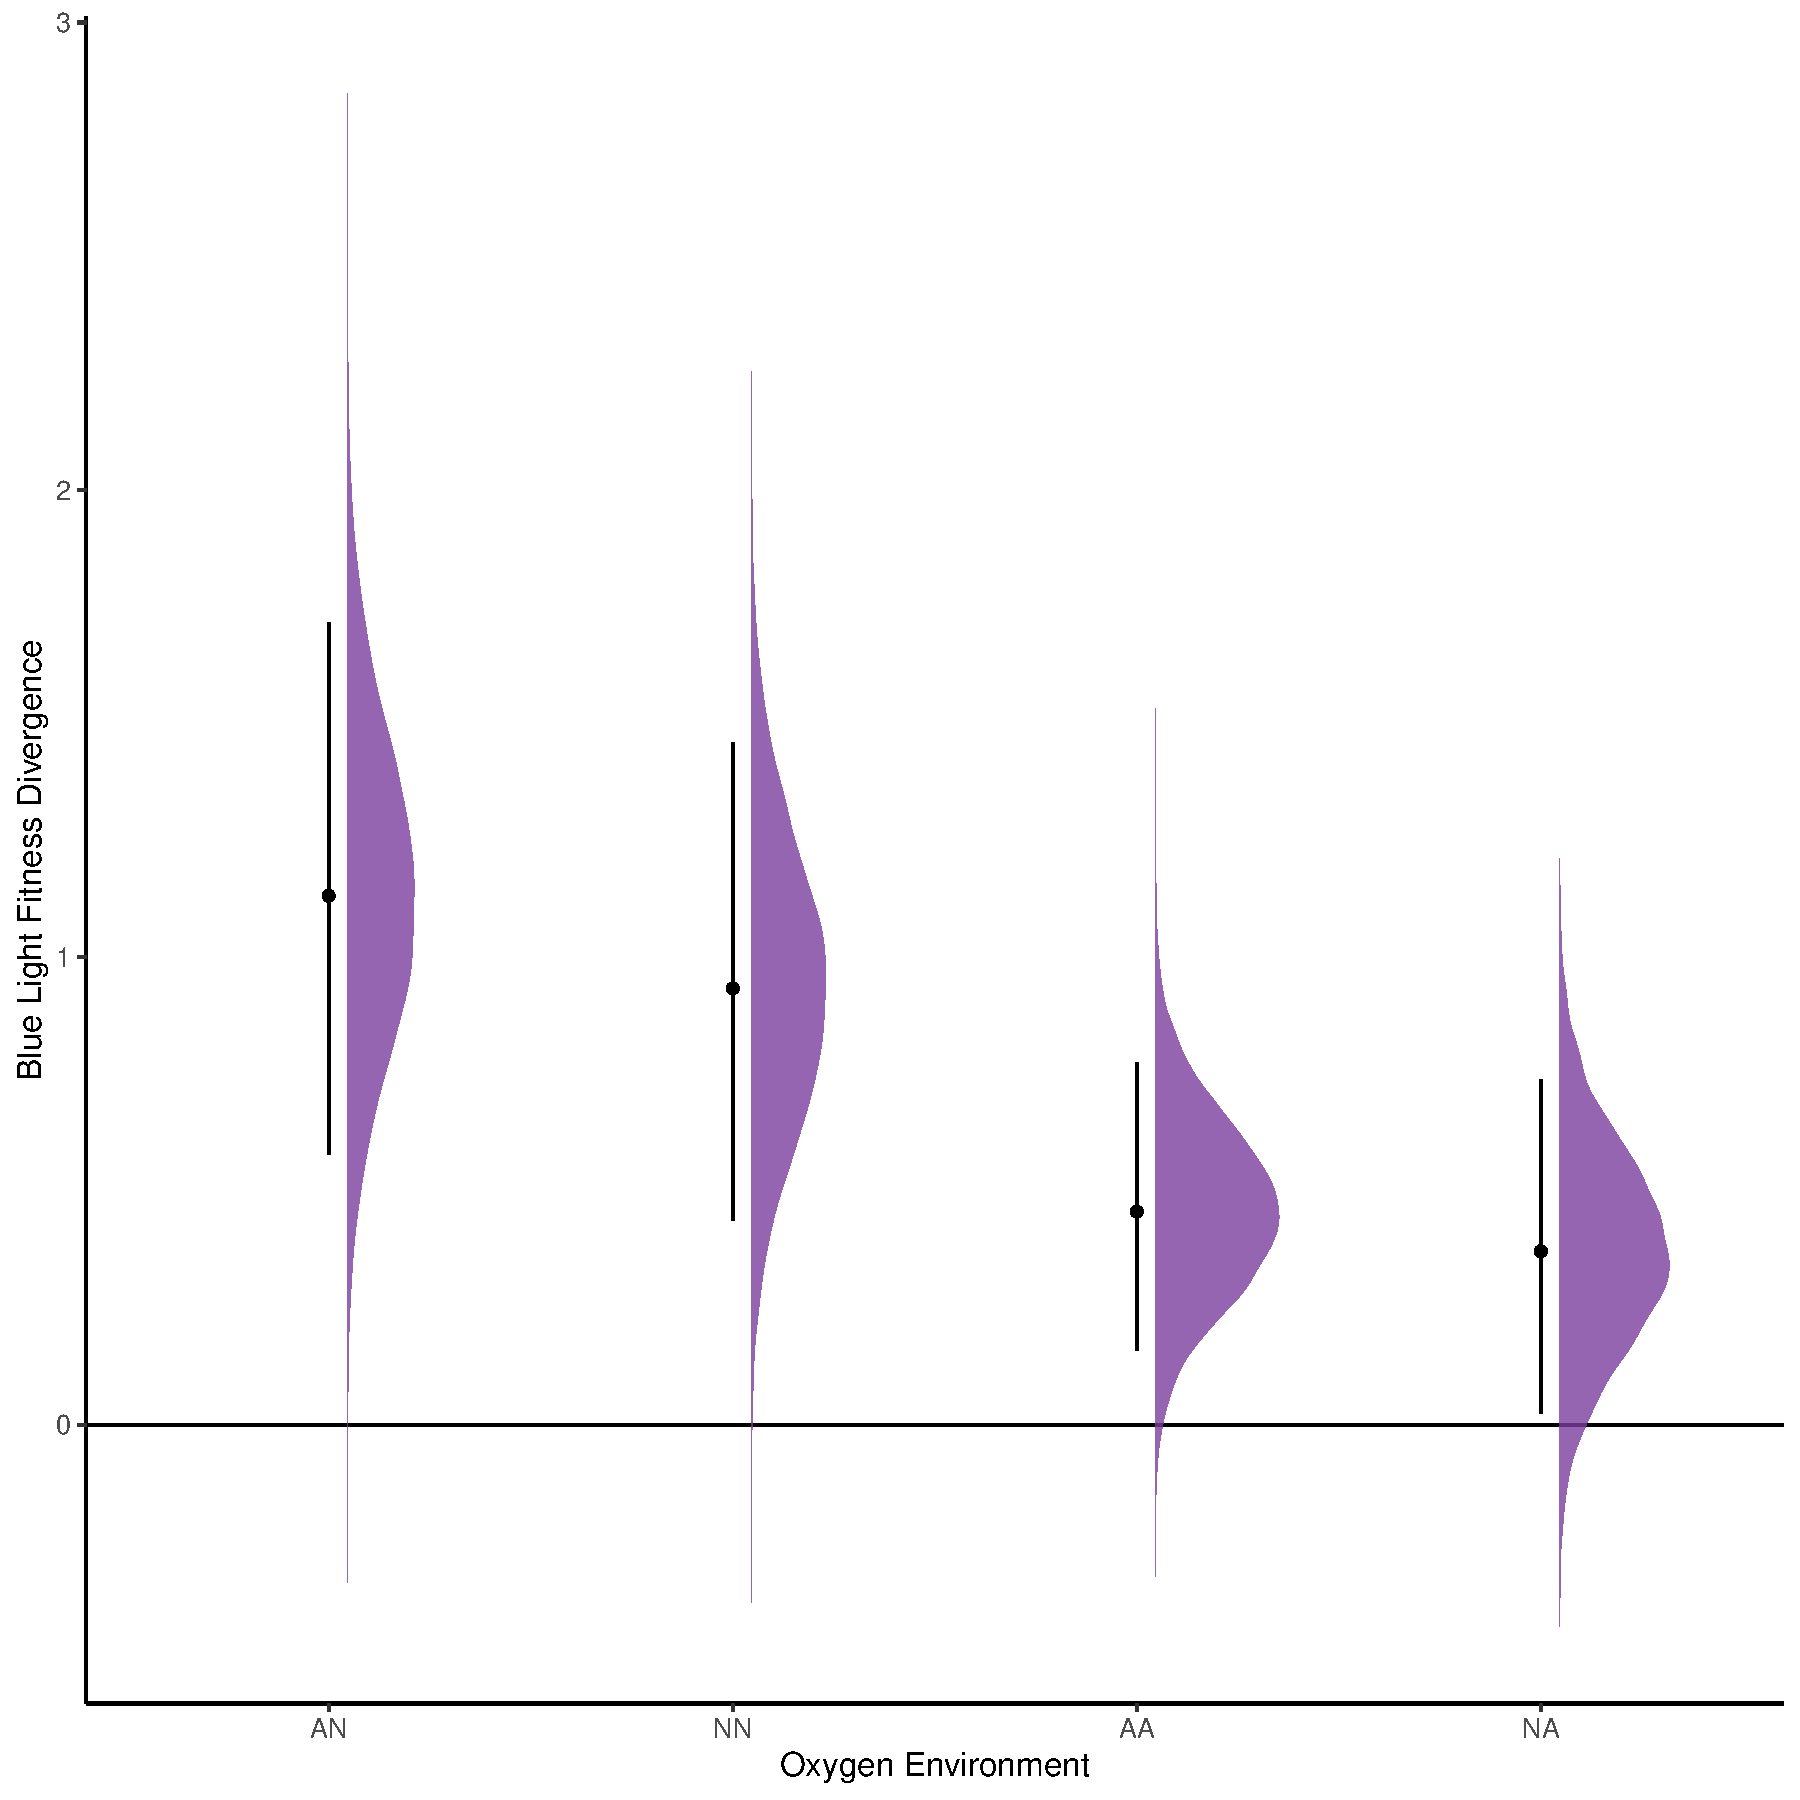
\includegraphics[keepaspectratio]{03_Combined_Growth_Fecundity_Plots_files/figure-latex/growth_plot_rel_vs_unrel_blue_light_diff -1.pdf}}

\pandocbounded{\includegraphics[keepaspectratio]{03_Combined_Growth_Fecundity_Plots_files/figure-latex/growth_plot_growth_variance_pairs_shared_pop-1.pdf}}

\subsubsection{Sequence specific fitness
estimates}\label{sequence-specific-fitness-estimates}

And now for the model with both Rel and Unrel fit at the same time.

\pandocbounded{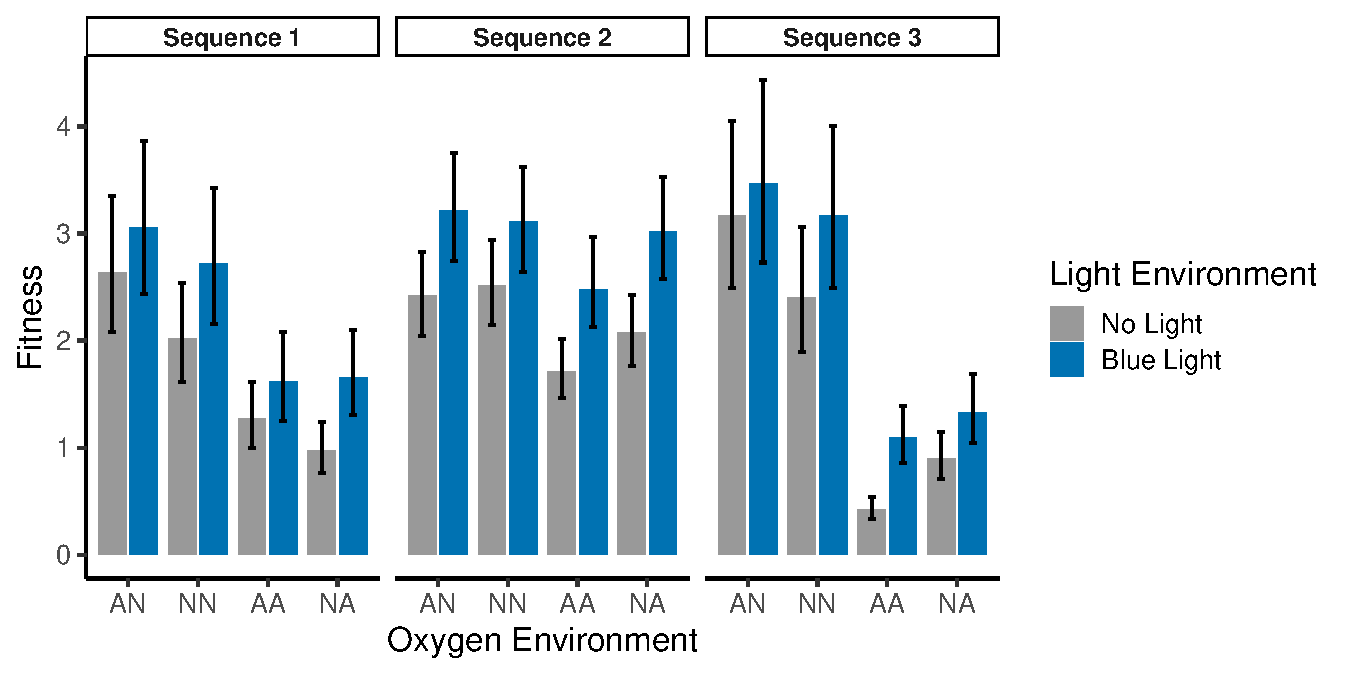
\includegraphics[keepaspectratio]{03_Combined_Growth_Fecundity_Plots_files/figure-latex/growth_plot_rel_by_sequence_matcue_intervals_state_only_from_full_model-1.pdf}}

\pandocbounded{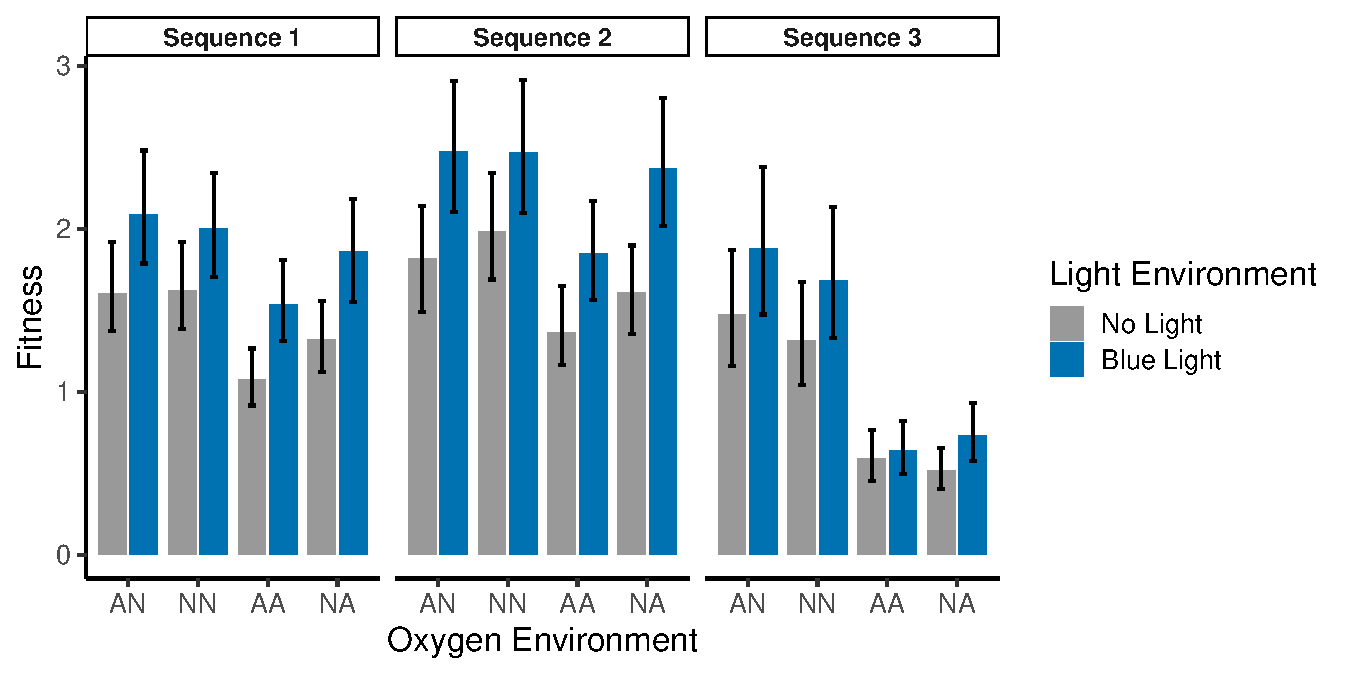
\includegraphics[keepaspectratio]{03_Combined_Growth_Fecundity_Plots_files/figure-latex/growth_plot_unrel_by_sequence_matcue_intervals_state_only_from_full_model-1.pdf}}

Plot the fitness divergence between Reliable and Unreliable by sequence.
To do this we average over maternal oxygen envirnoments and only take
the contrast the presence of blue light.

\pandocbounded{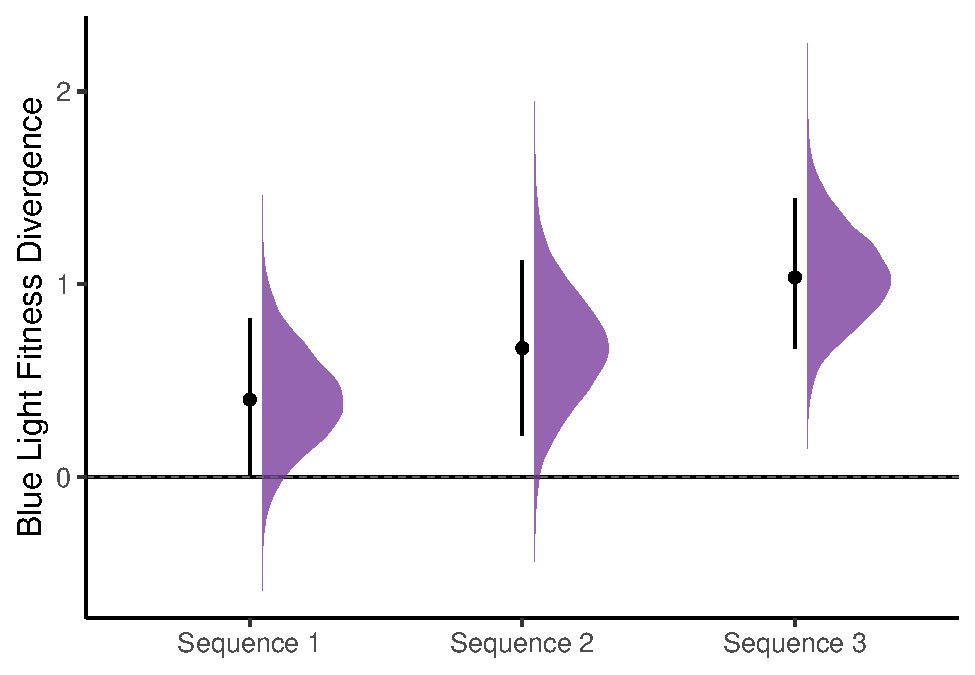
\includegraphics[keepaspectratio]{03_Combined_Growth_Fecundity_Plots_files/figure-latex/growth_plot_rel_minus_unrel_blue_only_by_sequence_from_full_model-1.pdf}}

Get prepared to plot the cue response divergence by maternal env for
each seq.

This is the contrast in cue response between reliable and unreliable on
the log scale.

\pandocbounded{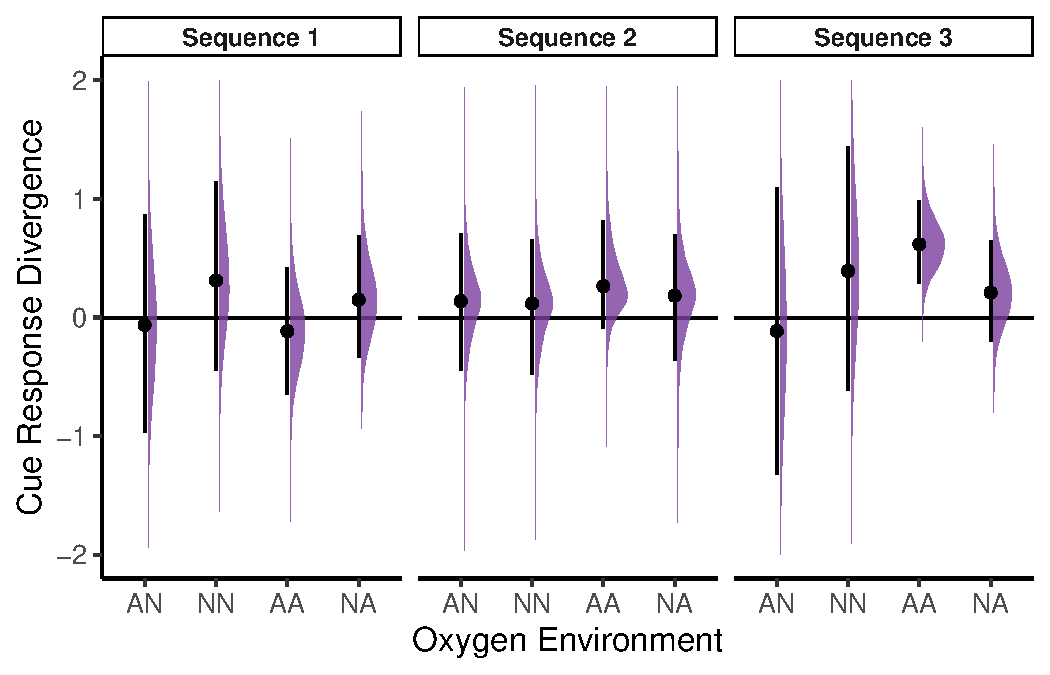
\includegraphics[keepaspectratio]{03_Combined_Growth_Fecundity_Plots_files/figure-latex/growth_plot_rel_minus_unrel_log_cue_contrast_by_sequence_from_full_model-1.pdf}}

\pandocbounded{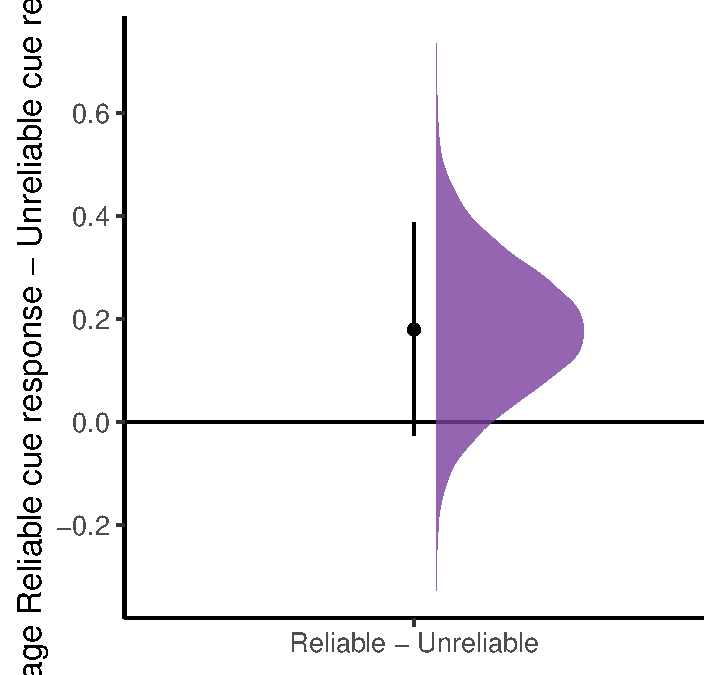
\includegraphics[keepaspectratio]{03_Combined_Growth_Fecundity_Plots_files/figure-latex/growth_plot_rel_minus_unrel_log_cue_contrast_average_from_full_model-1.pdf}}

now figure out exactly how much is below 0. The answer is 7.9\%.

\begin{Shaded}
\begin{Highlighting}[]
\NormalTok{plot\_df\_rel\_minus\_unrel\_log\_cue\_contrast\_avg }\SpecialCharTok{\%\textgreater{}\%}
\NormalTok{  dplyr}\SpecialCharTok{::}\FunctionTok{group\_by}\NormalTok{(contrast\_label) }\SpecialCharTok{\%\textgreater{}\%}
\NormalTok{  dplyr}\SpecialCharTok{::}\FunctionTok{summarise}\NormalTok{(}
    \AttributeTok{med =} \FunctionTok{median}\NormalTok{(rel\_minus\_unrel\_log\_cue\_contrast\_avg),}
    \AttributeTok{lo =} \FunctionTok{quantile}\NormalTok{(rel\_minus\_unrel\_log\_cue\_contrast\_avg, }\FloatTok{0.079}\NormalTok{),}
    \AttributeTok{hi =} \FunctionTok{quantile}\NormalTok{(rel\_minus\_unrel\_log\_cue\_contrast\_avg, growth\_hi\_p),}
    \AttributeTok{.groups =} \StringTok{"drop"}
\NormalTok{  )}
\end{Highlighting}
\end{Shaded}

\begin{verbatim}
## # A tibble: 1 x 4
##   contrast_label          med        lo    hi
##   <fct>                 <dbl>     <dbl> <dbl>
## 1 Reliable - Unreliable 0.180 -0.000532 0.389
\end{verbatim}

\subsection{Fecundity data}\label{fecundity-data}

\pandocbounded{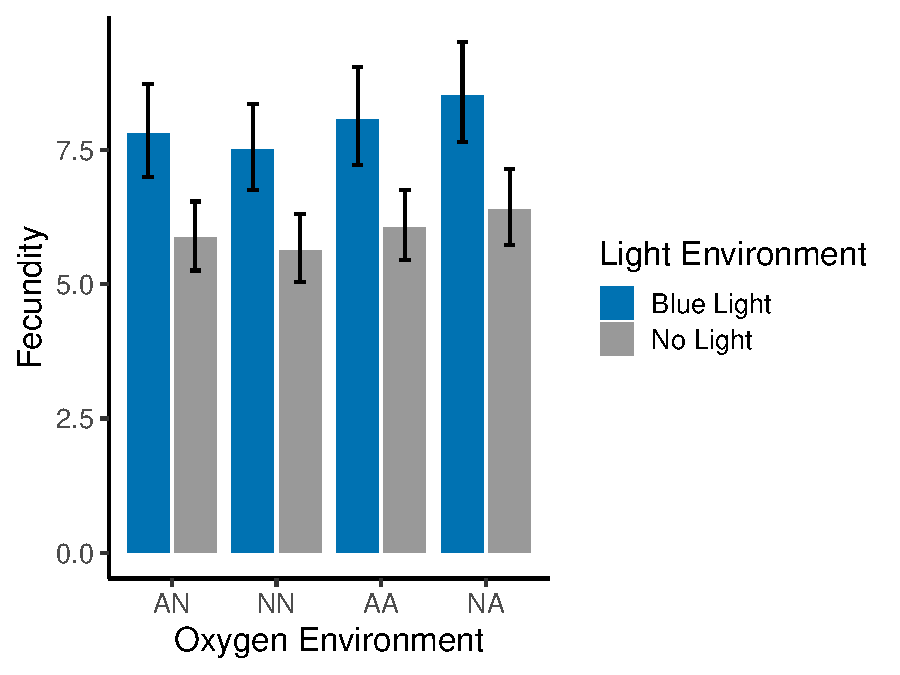
\includegraphics[keepaspectratio]{03_Combined_Growth_Fecundity_Plots_files/figure-latex/fec_plot_anc_fec_by_matcue_intervals_from_mat_and_cue_only-1.pdf}}

\pandocbounded{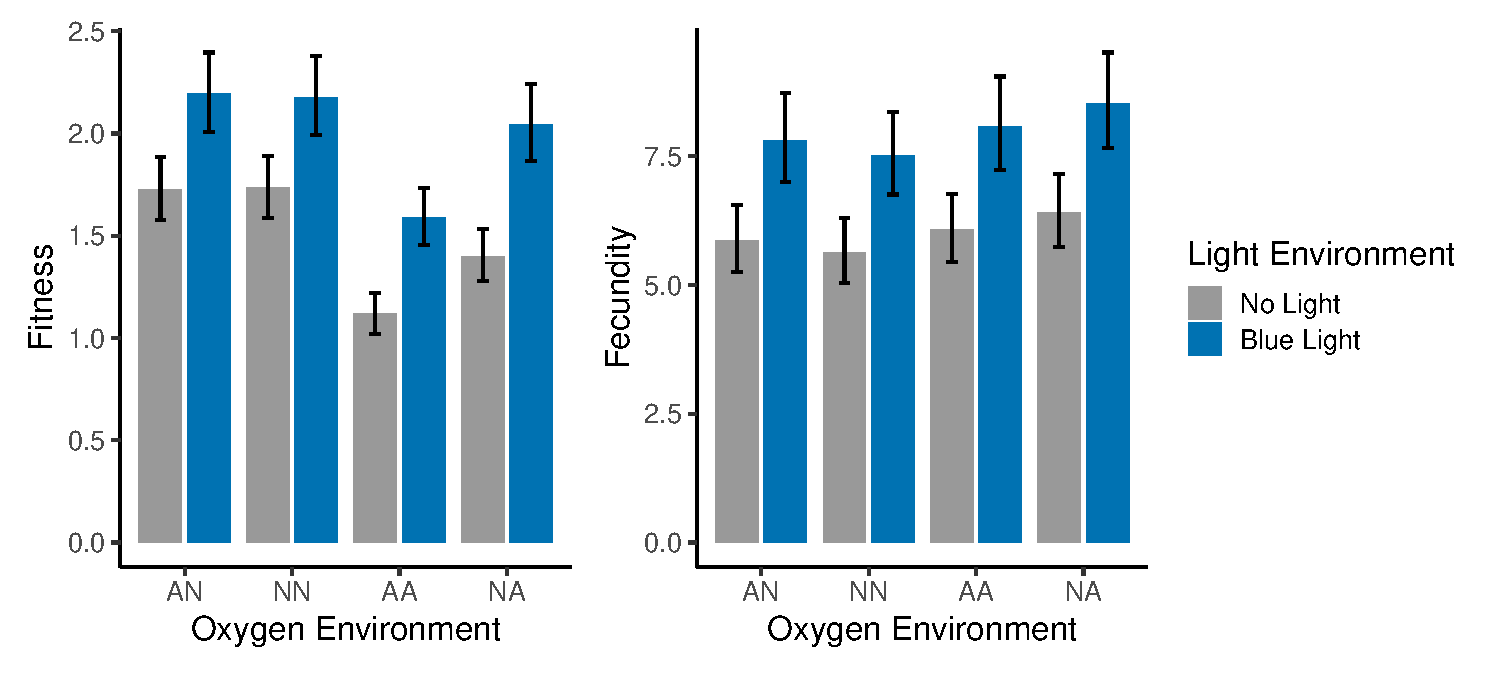
\includegraphics[keepaspectratio]{03_Combined_Growth_Fecundity_Plots_files/figure-latex/plot_anc_growth_and_fec_by_matcue_two_panel-1.pdf}}

\pandocbounded{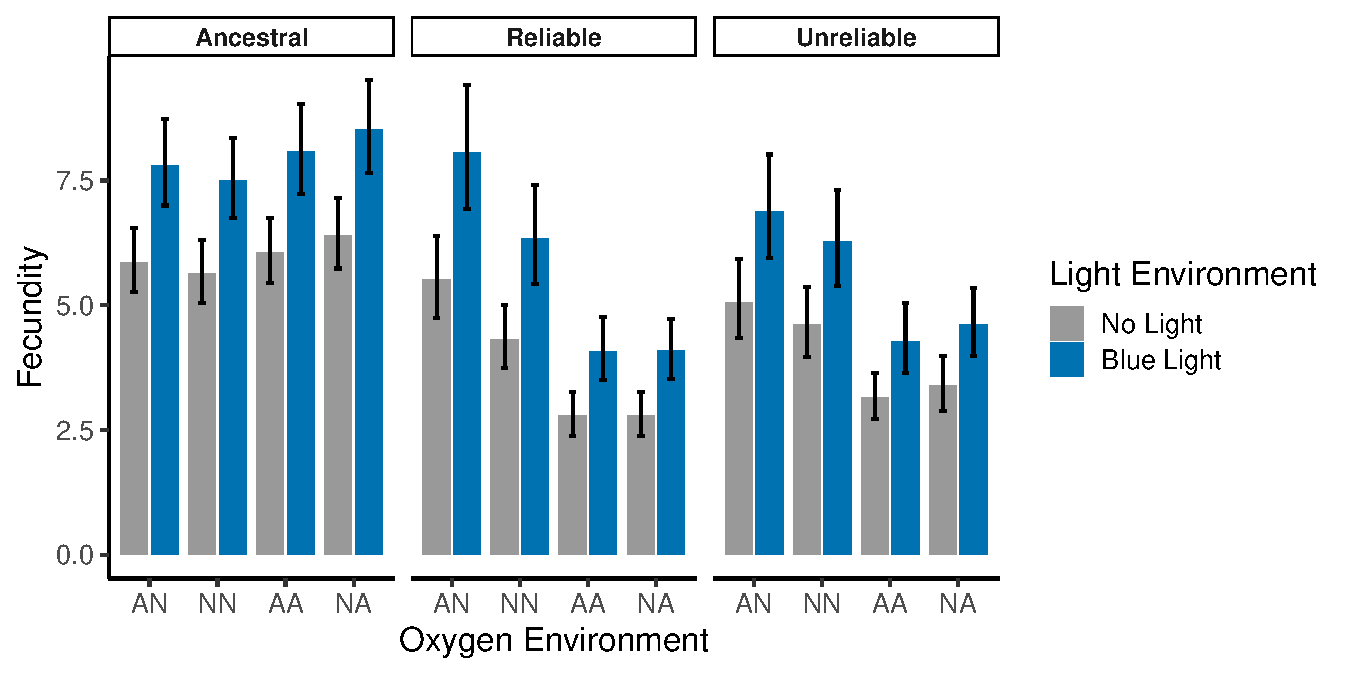
\includegraphics[keepaspectratio]{03_Combined_Growth_Fecundity_Plots_files/figure-latex/fec_plot_all_fec_by_matcue_intervals_from_mat_and_cue_only-1.pdf}}

\pandocbounded{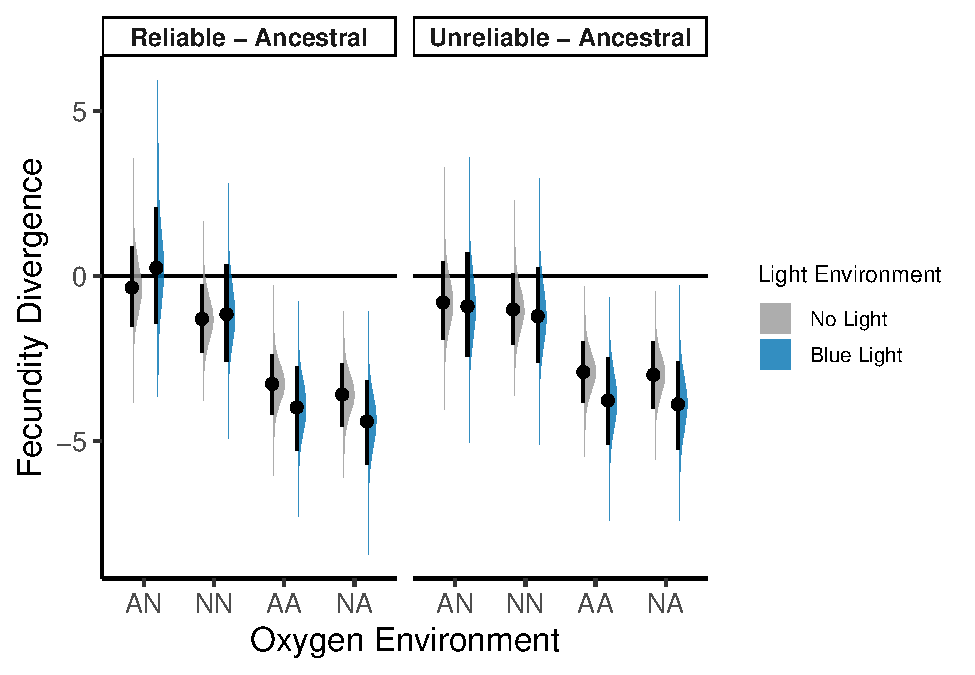
\includegraphics[keepaspectratio]{03_Combined_Growth_Fecundity_Plots_files/figure-latex/fec_plot_difference_anc_vs_rel_unrel_matcue_only-1.pdf}}

\pandocbounded{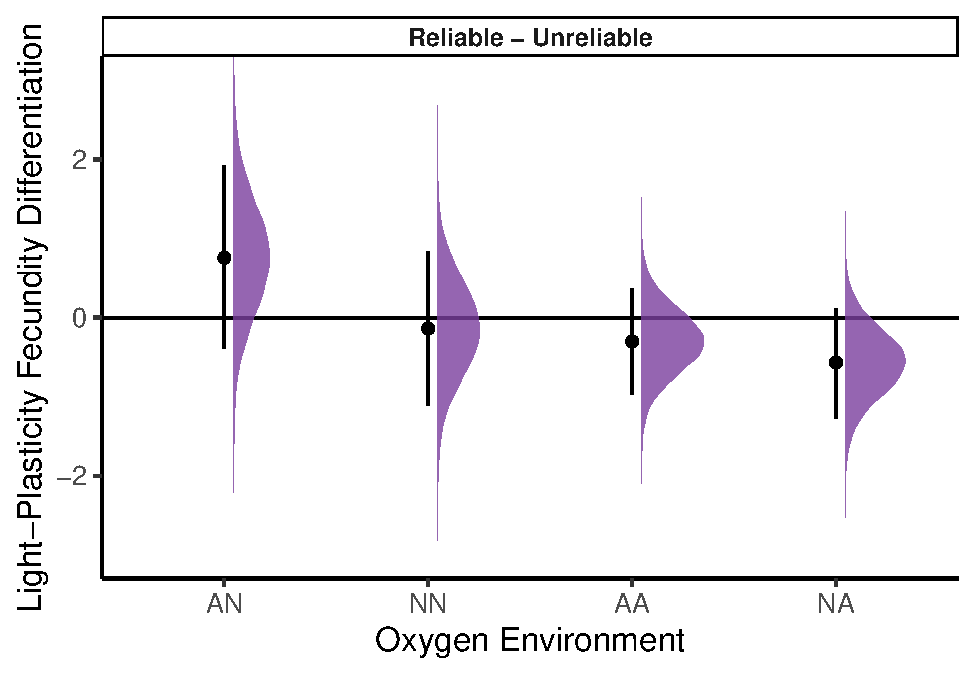
\includegraphics[keepaspectratio]{03_Combined_Growth_Fecundity_Plots_files/figure-latex/fec_plot_rel_minus_unrel_mat_only-1.pdf}}

\pandocbounded{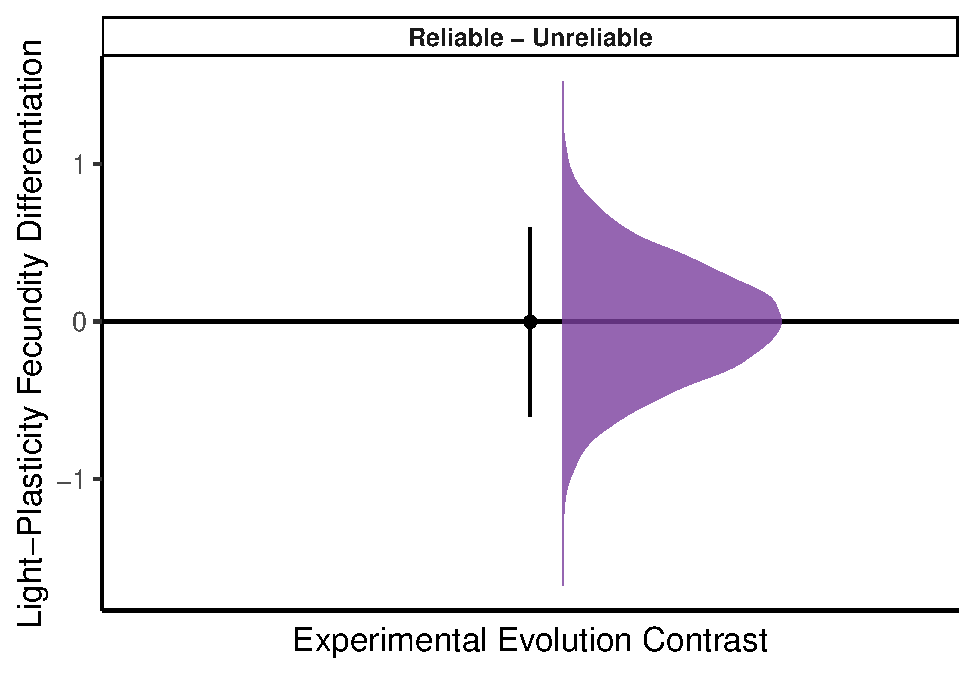
\includegraphics[keepaspectratio]{03_Combined_Growth_Fecundity_Plots_files/figure-latex/fec_plot_rel_minus_unrel_cue_only-1.pdf}}

\pandocbounded{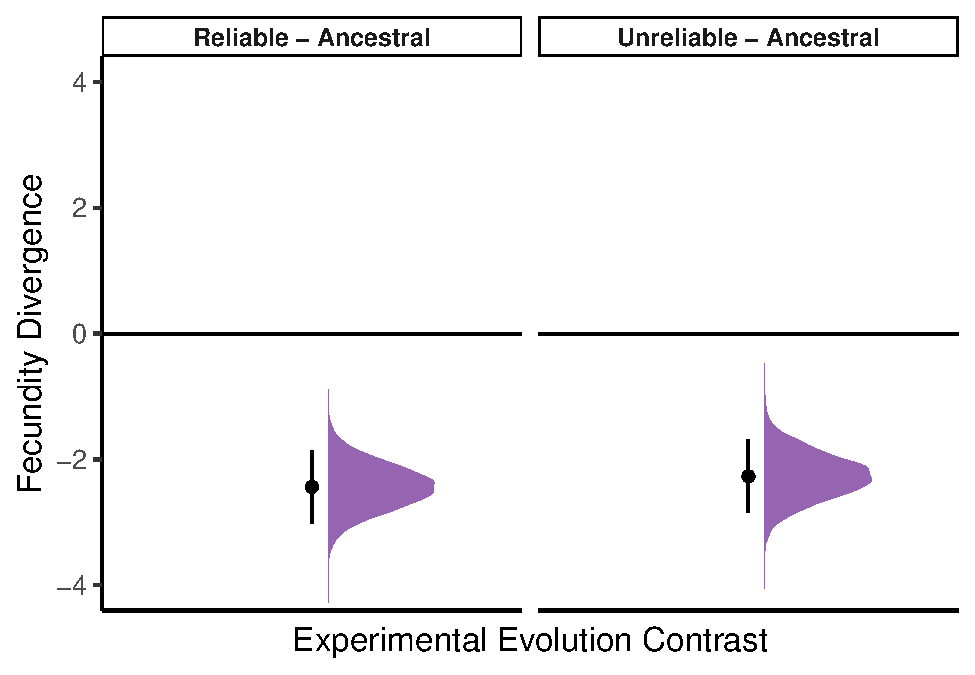
\includegraphics[keepaspectratio]{03_Combined_Growth_Fecundity_Plots_files/figure-latex/fec_plot_difference_anc_vs_rel_unrel_intercept_only-1.pdf}}

\pandocbounded{\includegraphics[keepaspectratio]{03_Combined_Growth_Fecundity_Plots_files/figure-latex/fec_plot_fecundity_variance_pairs_shared_pop-1.pdf}}

\end{document}
